% Bayes purity identity (prop. thm:bayes-purity), symmetric operating point TPR = 1 - FPR = alpha.
\begin{figure}[!htbp]
\centering
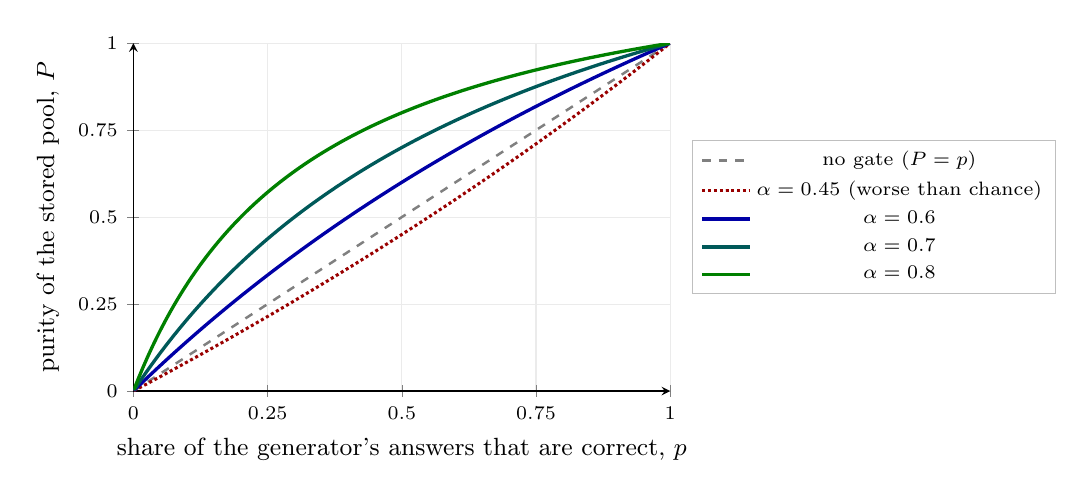
\begin{tikzpicture}
\begin{axis}[
  width=8.4cm, height=6.0cm,
  xlabel={share of the generator's answers that are correct, $p$},
  ylabel={purity of the stored pool, $P$},
  xmin=0, xmax=1, ymin=0, ymax=1,
  xtick={0,0.25,0.5,0.75,1}, ytick={0,0.25,0.5,0.75,1},
  axis lines=left, font=\small, tick label style={font=\scriptsize},
  legend style={at={(1.04,0.5)}, anchor=west, draw=black!25, font=\scriptsize, fill=white},
  grid=both, grid style={black!8}, domain=0.001:0.999, samples=120,
]
  \addplot[black!50, dashed, line width=0.9pt] {x}; \addlegendentry{no gate ($P = p$)}
  \addplot[red!60!black, line width=1.1pt, densely dotted] {0.45*x/(0.45*x + 0.55*(1-x))}; \addlegendentry{$\alpha = 0.45$ (worse than chance)}
  \addplot[blue!65!black, line width=1.2pt] {0.6*x/(0.6*x + 0.4*(1-x))}; \addlegendentry{$\alpha = 0.6$}
  \addplot[teal!70!black, line width=1.2pt] {0.7*x/(0.7*x + 0.3*(1-x))}; \addlegendentry{$\alpha = 0.7$}
  \addplot[green!50!black, line width=1.2pt] {0.8*x/(0.8*x + 0.2*(1-x))}; \addlegendentry{$\alpha = 0.8$}
\end{axis}
\end{tikzpicture}
\caption[How the purity of the stored pool depends on the gate's balanced accuracy.]{How the purity of the stored pool depends on the gate's balanced accuracy $\alpha$, from \Cref{eq:bayes-purity} with $\mathrm{TPR} = 1 - \mathrm{FPR} = \alpha$. Curves above the diagonal ($\alpha > 1/2$) make the pool purer than the generator; the dotted curve ($\alpha < 1/2$) makes it dirtier.}
\label{fig:purity-curves}
\end{figure}
